% Slides for 2024-02-07
% To create a slide, use the following:
% \begin{frame}{TITLE}
%     BODY
% \end{frame}

% To create a slide with a bullet list, use the following:
% \begin{frame}{TITLE}
%     \begin{itemize}
%         \item ITEM 1
%         \item ITEM 2
%     \end{itemize}    
% \end{frame}

% To create a slide with numbered list, use the following:
% \begin{frame}{TITLE}
%     \begin{enumerate}
%         \item ITEM 1
%         \item ITEM 2
%     \end{enumerate}
% \end{frame}

% To create a slide with a graphic:
% 1. Add the graphic to this folder (named picture.png)
% 2. Use the following:
% \begin{frame}{TITLE}
%     \centering
%     \includegraphics[height=0.7\textheight,width=0.7\textwidth,keepaspectratio]{picture.png}
% \end{frame}

% To create a slide with two columns, use the following:
% \begin{frame}{TITLE}
%     \begin{columns}
%         \begin{column}{0.5\textwidth}
%             COLUMN 1 BODY
%         \end{column}
%         \begin{column}{0.5\textwidth}
%             COLUMN 2 BODY
%         \end{column}
%     \end{columns}
% \end{frame}

\begin{frame}{Docker Compose for Entire App}
\end{frame}

\begin{frame}{NDVI-Normalized Difference Vegetation Index change between 2015-2021}
    \centering
    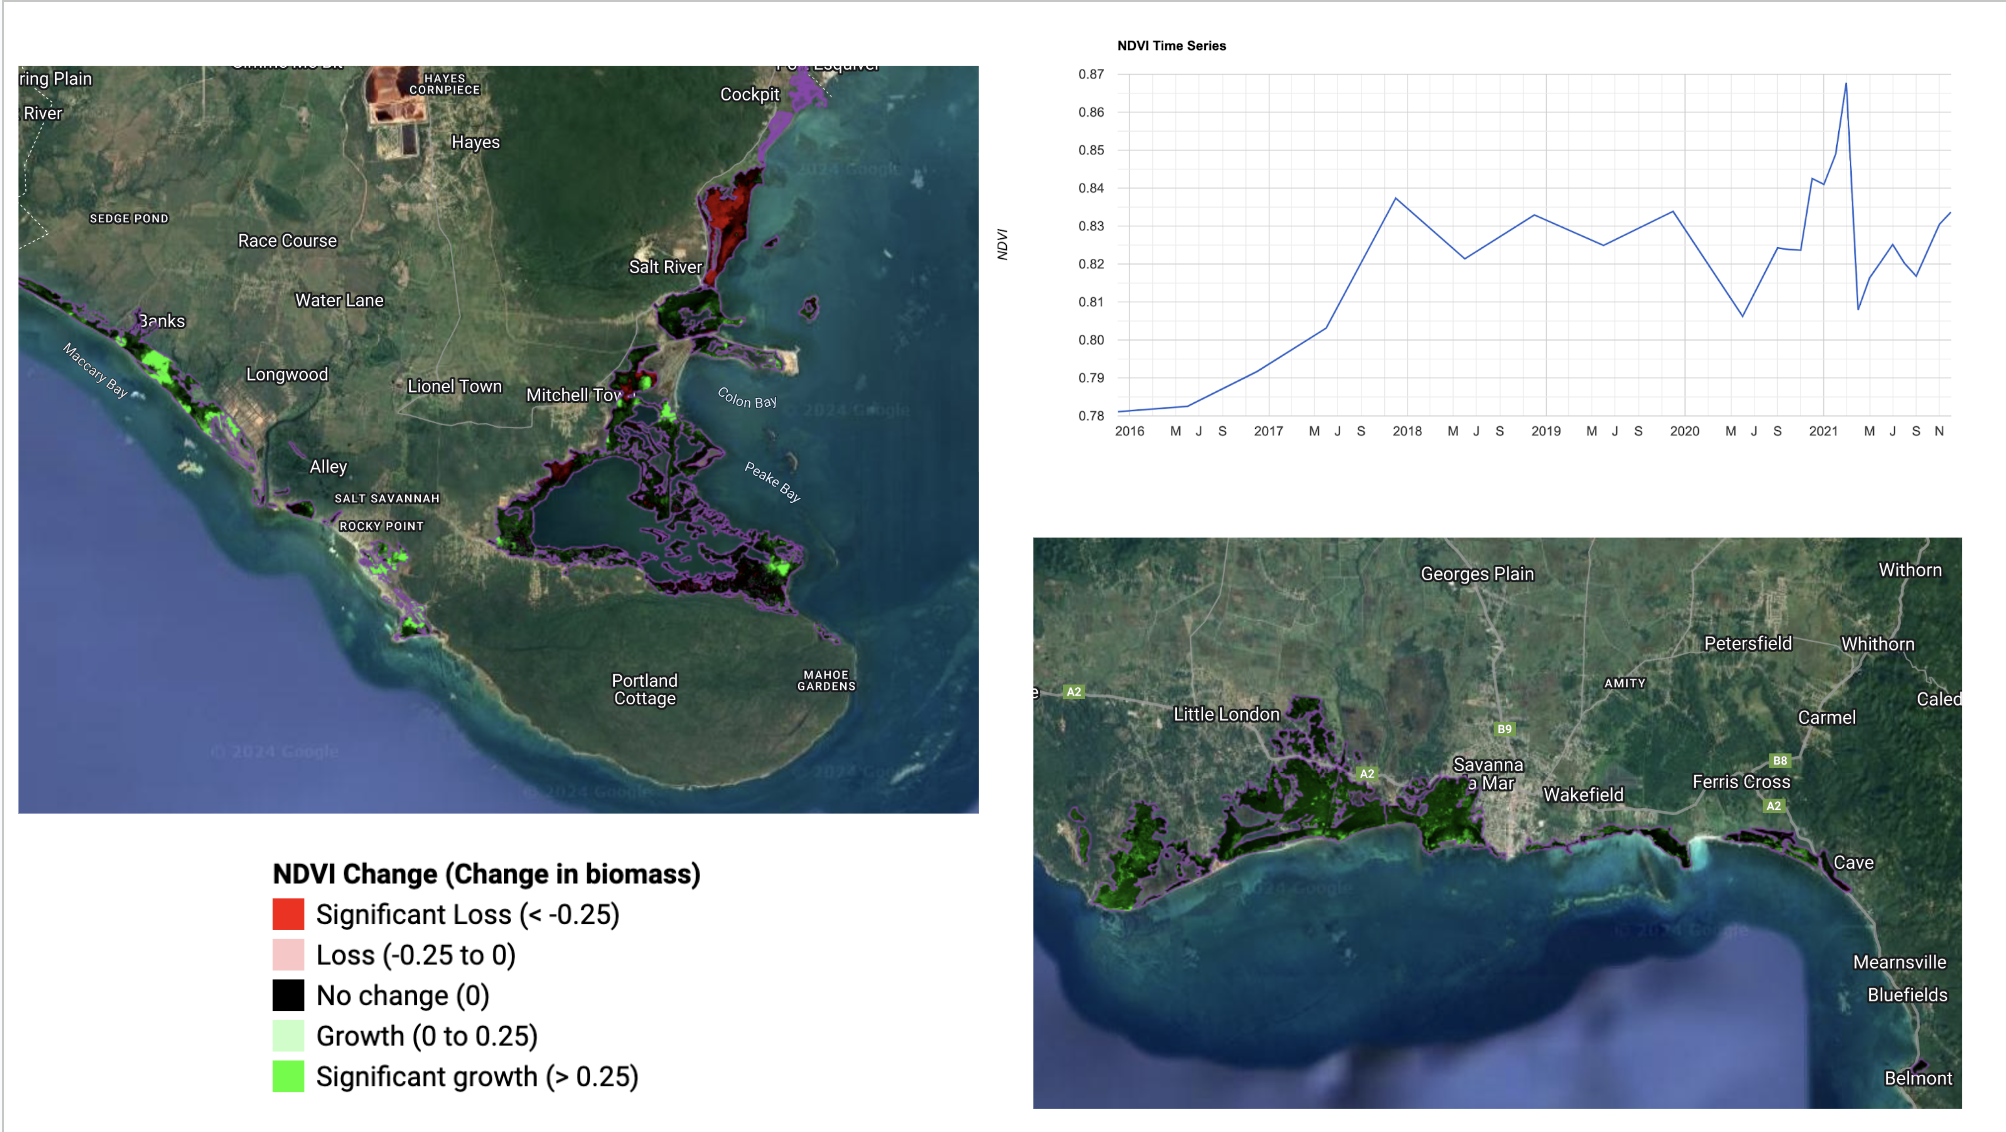
\includegraphics[height=0.7\textheight,width=0.7\textwidth,keepaspectratio]{mm-images/ndvi.png}
\end{frame}

\begin{frame}{Georeferenced Model Output}
    \centering
    \includegraphics[height=0.7\textheight,width=0.7\textwidth,keepaspectratio]{mm-images/tiffs.png}
\end{frame}

\begin{frame}{Image Processing with Satellite Imagery}
    Encoding channels into xarray.Dataset?  
\end{frame}

\begin{frame}{Copernicus Satellite Data}
    \begin{itemize}
        \item Request band data
        \item Calculate features
    \end{itemize}    
\end{frame}

\begin{frame}{User Upload Pipeline}
    \centering
    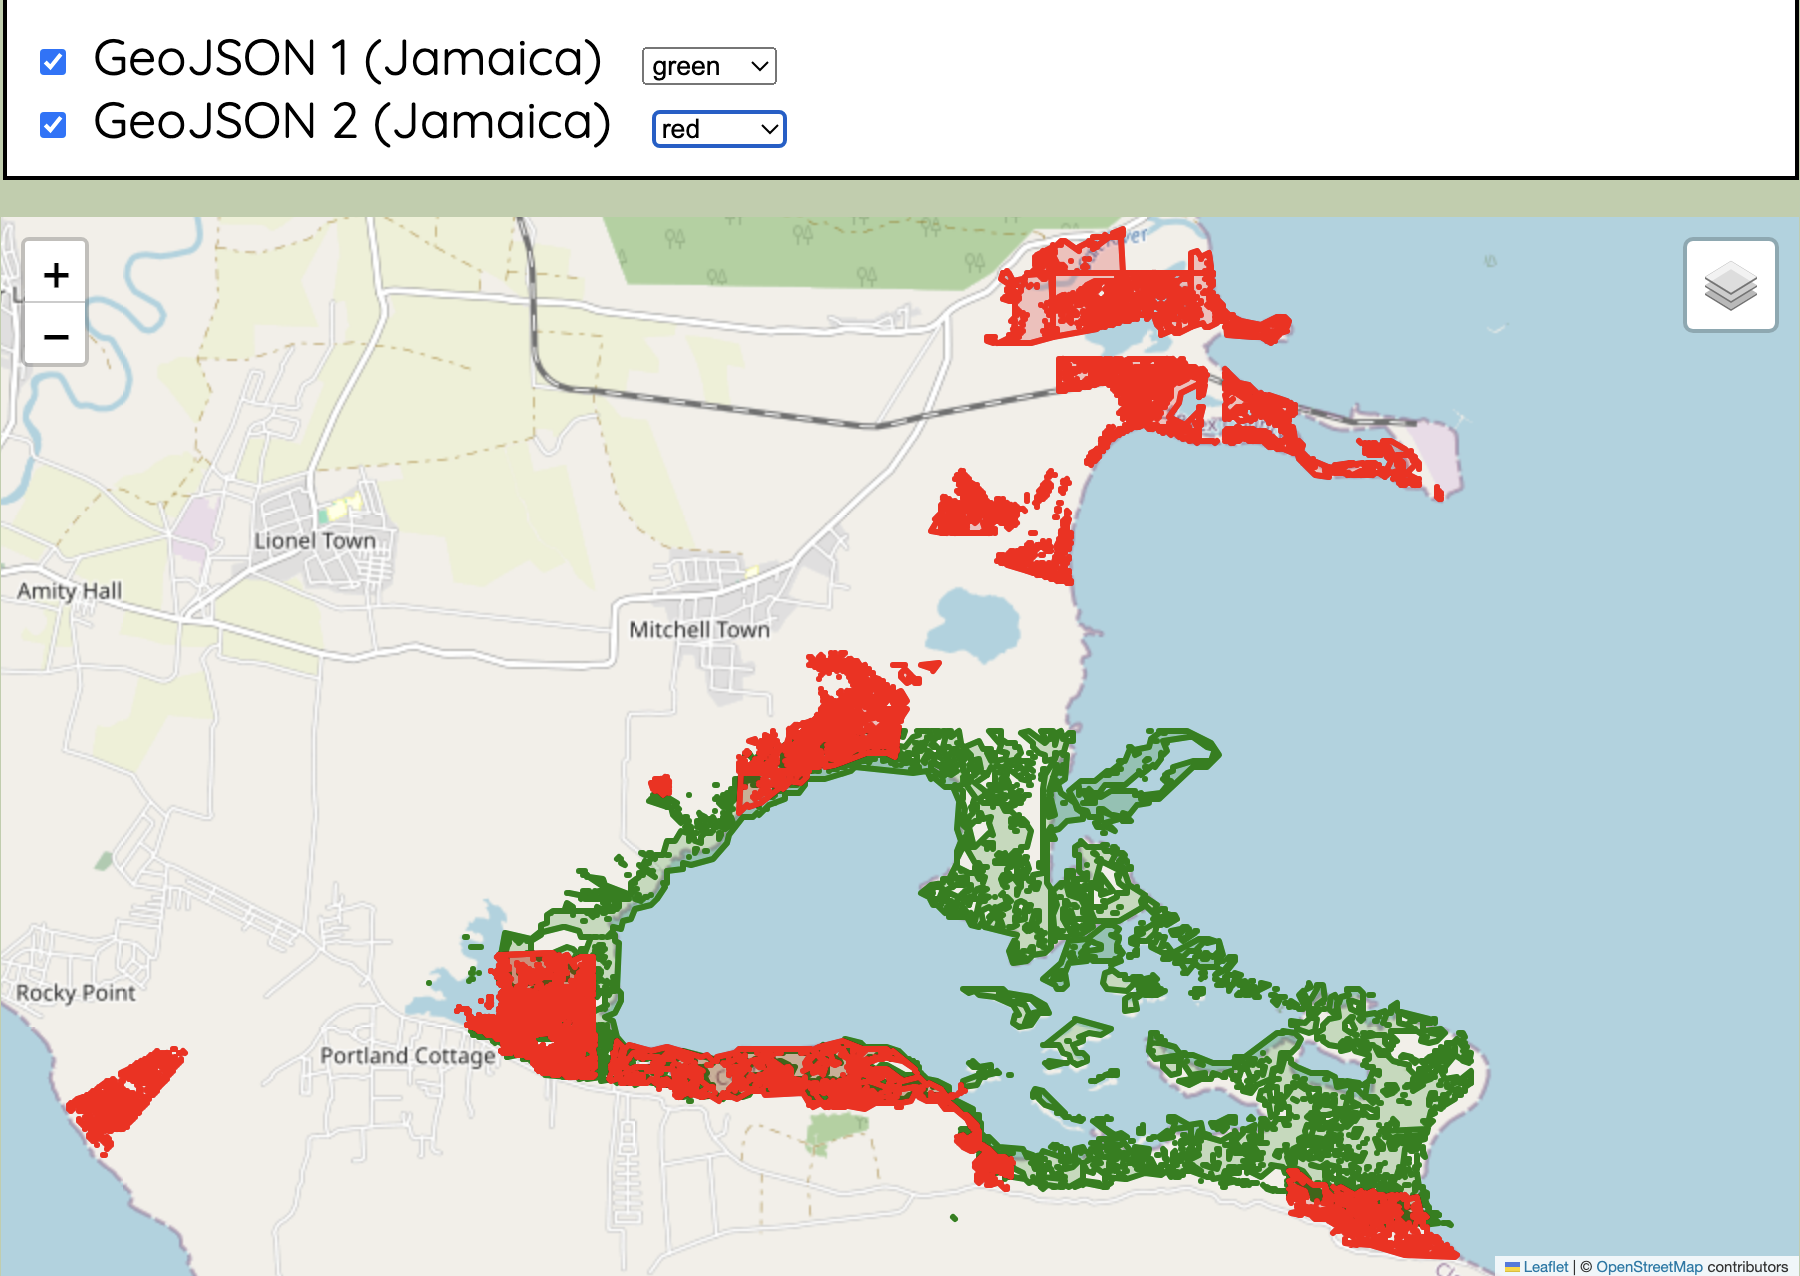
\includegraphics[height=0.7\textheight,width=0.7\textwidth,keepaspectratio]{mm-images/geojson-colors.png}
\end{frame}

\begin{frame}{Misc. Frontend}
    Reworked state for selecting color
    \centering
    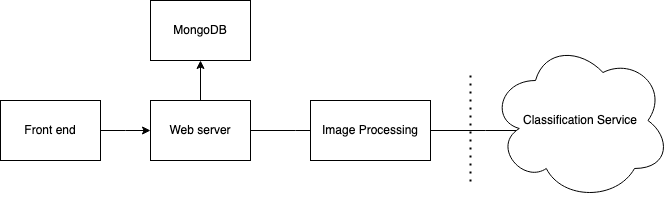
\includegraphics[height=0.7\textheight,width=0.7\textwidth,keepaspectratio]{mm-images/mongo-in-components.png}
\end{frame}